
% header %{{{1

\documentclass[tikz, border=1mm]{standalone}

\usepackage{amsmath}

\usepackage{tikz}
\usepackage[x11names]{xcolor}

\usetikzlibrary{calc,angles,quotes,shapes.geometric}

\usepackage{tkz-euclide}

\definecolor{goldenbrown}{HTML}{5b3c11}

% document %{{{1

% opening %{{{2

\begin{document}
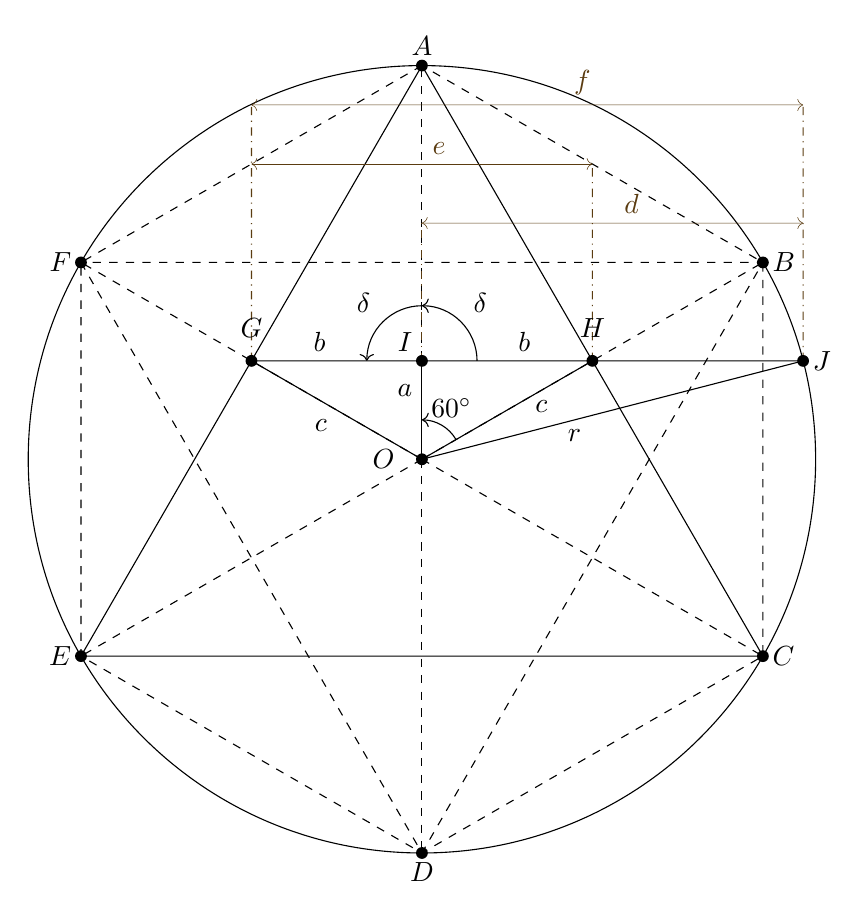
\begin{tikzpicture}[scale=2.5]

% parameters %{{{2

	\def\numsides{6}
	\def\radius{2}
	\def\rotation{90}

% coordinates %{{{2

	\coordinate (O) at (0,0);
	\foreach \i in {1,...,\numsides} {
		\coordinate (P\i) at ({360/\numsides*(\i-1)+\rotation}:\radius);
	}

% intersections %{{{2

	\tkzInterLL(O,P2)(P1,P3)\tkzGetPoint{G}
	\tkzInterLL(O,P6)(P1,P5)\tkzGetPoint{H}
	\tkzInterLL(O,P1)(G,H)\tkzGetPoint{I}

	\tkzInterLC(G,H)(O,P1)\tkzGetFirstPoint{J}

% coordinates for dimension lines %{{{

	\coordinate (IdJ) at ($(I) + (0,0.7)$);
	\coordinate (JdI) at ($(J) + (0,0.7)$);

	\coordinate (GdH) at ($(G) + (0,1.0)$);
	\coordinate (HdG) at ($(H) + (0,1.0)$);

	\coordinate (GdJ) at ($(G) + (0,1.3)$);
	\coordinate (JdG) at ($(J) + (0,1.3)$);

% circle %{{{2

	\draw (O) circle (\radius);

% polygon %{{{2

	\draw[dashed] (P1) \foreach \i in {2,...,\numsides} { -- (P\i) } -- cycle;

% radiuses %{{{2

	\draw[dashed] (O) -- (P1);
	\draw[dashed] (O) -- (P2);
	\draw[dashed] (O) -- (P3);
	\draw[dashed] (O) -- (P4);
	\draw[dashed] (O) -- (P5);
	\draw[dashed] (O) -- (P6);

% hexagram %{{{2

	\draw (P1) -- (P3) -- (P5) -- cycle;
	\draw[dashed] (P2) -- (P4) -- (P6) -- cycle;

% other lines %{{{2

	\draw (O) -- (G);
	\draw (O) -- (I);
	\draw (O) -- (H);
	\draw (O) -- (J);

	\draw (G) -- (J);

% dimension lines %{{{2

	\draw[<->, line width=0.2pt, goldenbrown] (IdJ) -- (JdI);
	\draw[dashdotted, goldenbrown] (I) -- (IdJ);
	%\draw[dashdotted, goldenbrown] (J) -- (JdI);

	\draw[<->, line width=0.2pt, goldenbrown] (GdH) -- (HdG);
	%\draw[dashdotted, goldenbrown] (G) -- (GdH);
	\draw[dashdotted, goldenbrown] (H) -- (HdG);

	\draw[<->, line width=0.2pt, goldenbrown] (GdJ) -- (JdG);
	\draw[dashdotted, goldenbrown] (G) -- (GdJ);
	\draw[dashdotted, goldenbrown] (J) -- (JdG);

% points, dots, vertices labels %{{{

	\fill (O) circle (0.3mm);
	\fill (G) circle (0.3mm);
	\fill (H) circle (0.3mm);
	\fill (I) circle (0.3mm);
	\fill (J) circle (0.3mm);
	\foreach \i in {1,...,\numsides} { \fill (P\i) circle (0.3mm); }

% points, dots, vertices labels %{{{2

	\node[label={[label distance=1.0mm]left:$O$}] at (O) {};

	\node[above] at (P1) {$A$};
	\node[right] at (P6) {$B$};
	\node[right] at (P5) {$C$};
	\node[below] at (P4) {$D$};
	\node[left] at (P3) {$E$};
	\node[left] at (P2) {$F$};

	\node[label={[label distance=0.5mm]above:$G$}] at (G) {};
	\node[label={[label distance=0.5mm]above:$H$}] at (H) {};
	\node[above left] at (I) {$I$};
	\node[right] at (J) {$J$};

% segments labels %{{{2

	\node[left] at ($(O)!0.7!(I)$) {$a$};
	\node[above] at ($(G)!0.4!(I)$) {$b$};
	\node[above] at ($(I)!0.6!(H)$) {$b$};
	\node[below left] at ($(O)!0.5!(G)$) {$c$};
	\node[below] at ($(O)!0.7!(H)$) {$c$};
	\node[below] at ($(O)!0.4!(J)$) {$r$};

	\node[above, goldenbrown] at ($(IdJ)!0.55!(JdI)$) {$d$};
	\node[above, goldenbrown] at ($(GdH)!0.55!(HdG)$) {$e$};
	\node[above, goldenbrown] at ($(GdJ)!0.6!(JdG)$) {$f$};

% angles labels %{{{2

	\pic[draw, ->, "$60^\circ$", angle radius=0.5cm, angle eccentricity=1.5]
	{angle = H--O--I};

	\pic[draw, ->, "$\delta$", angle radius=0.7cm, angle eccentricity=1.5]
	{angle = P1--I--G};

	\pic[draw, ->, "$\delta$", angle radius=0.7cm, angle eccentricity=1.5]
	{angle = H--I--P1};

% closing %{{{2

\end{tikzpicture}
\end{document}
